\subsection{Overview}

% Faire le cycle du petrole
Into the depth of the Earth, petroleum and natural gas are trapped.
%
These sources of energy are the result of the transformation of organic matter coming from vegetables and dead animals under very high constraint during millions of years.
%
Hardly hide under several kilometers of stone, petroleum companies, as Total S.A., tried to find them all, before a concurrent company.



More generally, we call reservoir of hydrocarbon, or shorter just reservoir, a major concentration of petroleum and/or natural gas under the ground.
%
The first step to find a reservoir is to analyze the underground with seismic waves.
%
These waves are generated by bomb for under sea analysis or with seismic truck for Earth's surface.
%
When these seismic waves are analyzed with some waves equation modeling software, petroleum companies can obtain a pretty good representation of the underground.
%
When a reservoir is found, one of the first questions is : "Does it pay to exploit this reservoir ?".
%
Reservoir simulations help to answer this question.
%
By doing a flow of fluid simulation through porous media, petroleum companies can obtain an approximation of the among of possible oil recovering.
%
If it is profitable to exploit the reservoir, petroleum companies can start exploiting the reservoir.



But it is not sufficient to dig and wait for petroleum sprung in a geyser form like we can see in animated cartoon.
%
Petroleum companies need to install some wells.
%
There are two major kinds of wells (Fig .\ref{fig:wells}) :
%
\begin{itemize}
  \item Producer wells,
  \item Injector wells,
\end{itemize}

%   (-_-)   %
\begin{figure}[!ht]
  \centering
  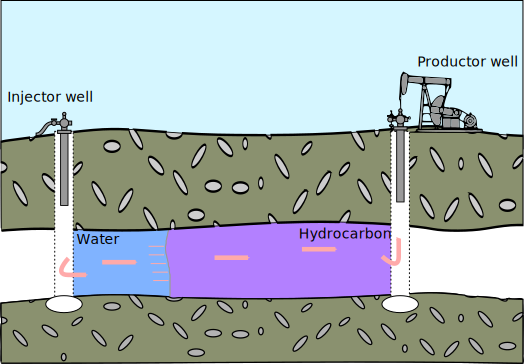
\includegraphics[width=0.8\textwidth]{wells}
  \caption{A field with two wells.}
\label{fig:wells}
\end{figure}


Reservoir engineers need to find the optimal number of wells and also their optimal placement.
%
Again, they use reservoir simulations to test different configurations.
%
Later, when the petroleum company start exploiting the field, it can be interesting to forecast oil production.
%
Once again, reservoir simulation helps (Fig. \ref{fig:floviz}).

%   (-_-)   %
\begin{figure}[!ht]
  \centering
  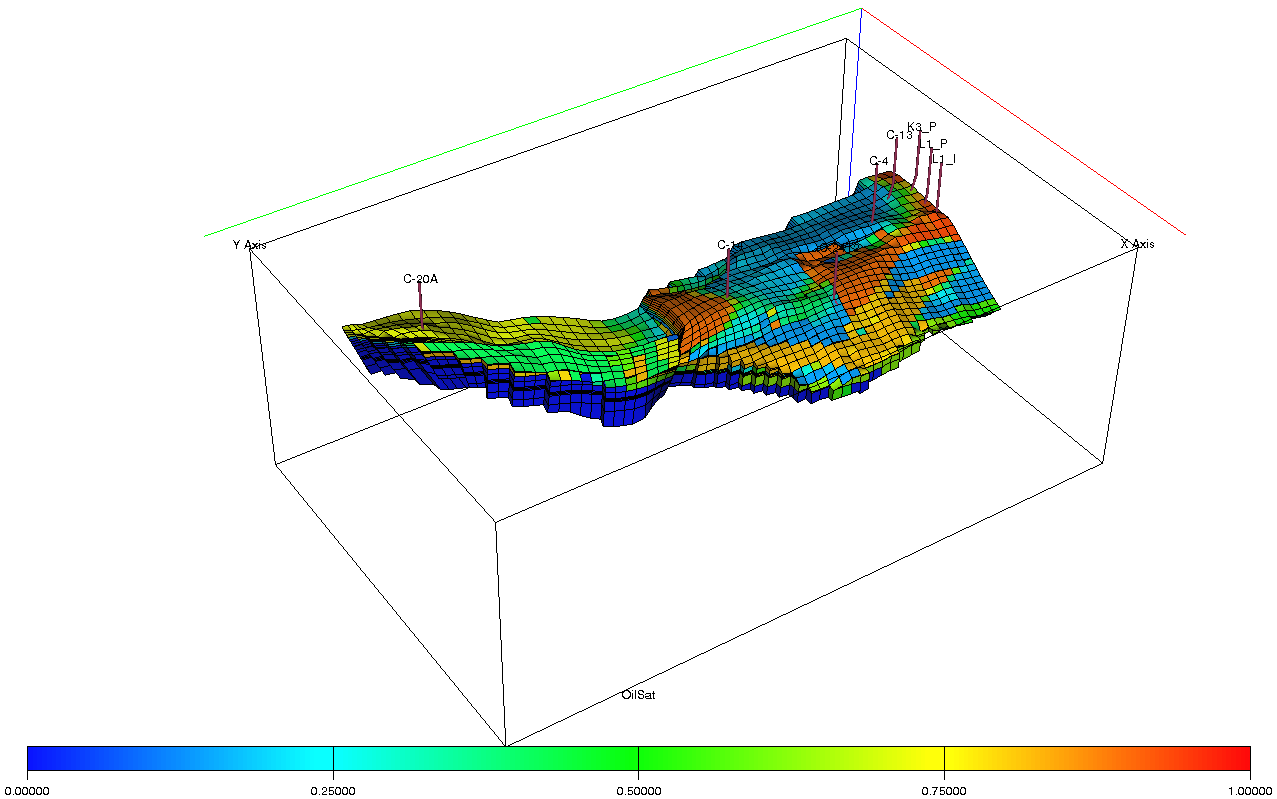
\includegraphics[width=\textwidth]{reservoir}
  \caption{Saturation of oil in a reservoir during a simulation.}
\label{fig:floviz}
\end{figure}


As shown previously, reservoir simulation is a key step in the oil recovery process.
%
Petroleum companies want to simulate more and more precisely internal state of a reservoir, and of course as quickly as possible.
%
Let's see the structure of a reservoir simulator.
